\documentclass{article}
\usepackage[preprint]{neurips_2026}
\usepackage[utf8]{inputenc}
\usepackage[T1]{fontenc}
\usepackage{hyperref}
\hypersetup{hidelinks}
\usepackage{url}
\usepackage{booktabs}
\usepackage{amsmath}
\usepackage{amsfonts}
\usepackage{graphicx}
\usepackage{microtype}

\title{From Byte Tokens to Verified Tool Use:\\
A Reproducible Local Language-Model Lab}
\author{Advanced Machine Learning Project\\
\texttt{zongyangbigpolo/AdvancedMachineLearningTask}}

\begin{document}
\maketitle

\begin{abstract}
We connect a byte-level tokenizer, a decoder Transformer, pretraining,
systems measurements, data cleaning, scaling extrapolation, post-training,
and verified tool use in a locally reproducible experiment collection.
A from-scratch 98.3-million-parameter model is trained for 1,500 updates on
Apple M4, reducing fixed-window validation cross-entropy from 8.9119 to
2.7503 while still producing repetitive text. Fifteen smaller models
support a fixed-token-budget scaling experiment: a largest-model hold-out
prediction has 0.8575\% relative error. On a separate constrained numeric
task, same-base supervised fine-tuning, direct preference optimization,
and verifier-reward policy gradients reach mean held-out accuracies of
90\%, 90\%, and 85\%. A learned three-action policy completes new
16-goal ledger episodes averaging 68.08 tool actions. Self-review adds
no success gain in ordinary episodes, but repairs deliberately corrupted
draft actions at twice the inference-call cost. The experiments cover
finite task domains and short training budgets on one Apple GPU.
Code, measurements, data snapshots, small model
bundles, screenshots, and large-checkpoint releases accompany the report.
\end{abstract}

\section{Problem and motivation}

An implementation can run without establishing that its mathematics,
learning signal, and evaluation agree. Our central problem is to build an
inspectable chain from raw text to externally verified actions. We ask
three questions:
(1) can custom tokenizer and model components support
100-million-scale parameter updates; (2) can controlled local comparisons
separate implementation speed, model-size effects, and training signals;
and (3) can a learned policy complete dependent tool actions without using
an answer-producing rule at inference time?

The project is organized by five deliverables rather than calendar weeks.
The public \emph{from-token-to-agent} project~\citep{referenceproject} informed the tokenizer and
size-pilot comparisons. Stanford CS336 provides related systems, scaling,
and alignment assignment specifications~\citep{cs336}.

\section{Implementation and experimental protocol}

\subsection{Tokenizer and decoder}

The tokenizer implements Byte Pair Encoding (BPE), beginning with 256 byte
symbols and an End of Sequence (EOS) symbol. Pair frequencies are counted
within Unicode-aware pieces; deterministic tie-breaking and ranked,
non-overlapping merges make saved rules reproducible. Encoding followed
by decoding preserves input text, including Chinese and emoji.

The decoder contains explicit linear projections, Root Mean Square
Normalization (RMSNorm), Rotary Position Embedding (RoPE), causal
Multi-Head Attention (MHA), Swish Gated Linear Units (SwiGLU), residual
connections, and tied input/output embeddings. Future positions are
masked. The token-level objective is
\begin{equation}
  \mathcal L_{\mathrm{LM}}=-\frac{1}{T}\sum_{t=1}^{T}
       \log p_\theta(x_{t+1}\mid x_{\leq t}).
\end{equation}
PyTorch supplies tensors, automatic differentiation, and AdamW.
Tests compare attention and cross-entropy to reference PyTorch
operators, check causality and gradients, overfit a fixed batch, and
compare uninterrupted CPU training with normal checkpoint restoration.

\subsection{Large-model run}

The architecture has vocabulary capacity 8,192, width 768, 12 layers,
12 attention heads, and feed-forward width 2,304: 98,323,200 parameters.
The TinyStories snapshot contains 512 training stories and 128 validation
stories, with documented whitespace normalization and
CDLA-Sharing-1.0 attribution~\citep{tinystories}.
Only training text fits the tokenizer; its realized vocabulary is 5,696.
The streams contain 172,991 and 39,574 tokens.

Training uses Metal Performance Shaders (MPS), 32-bit floating point,
batch size one, context 128, and 1,500 AdamW updates. The learning rate
peaks at $3\cdot10^{-4}$ after 50 warmup updates and follows cosine decay.
The sampled budget is 192,000 tokens. Evaluation uses 16 fixed,
potentially overlapping 128-token windows, not the full validation set.
A prior separate 100-update run demonstrates stop-and-resume behavior;
it is not concatenated with the new run.

\subsection{Systems measurements}

We compare explicit scaled dot-product attention against PyTorch Scaled
Dot-Product Attention (SDPA), including forward and backward passes.
We also implement a per-layer Key-Value (KV) cache with offset-correct
RoPE, chunked prefill, batch checks, and explicit context-overflow errors.
Cached logits are checked against full-prefix logits on CPU;
greedy outputs match on MPS.

After other training processes finish, measurements synchronize the GPU
before and after wall-clock timing, exclude two warmups, and report
medians and ranges. Attention uses seven repeats; decoding uses five.
No Triton kernel or multi-GPU experiment is reported: the selected host
has one Apple GPU and no compatible Triton/CUDA test device.

\subsection{Raw-data and scaling experiment}

We save a MediaWiki XML export of 16 specified Simple English
Wikipedia articles, including revision URLs and a raw-file hash.
Cleaning removes templates, references, markup, and selected tables;
malformed template input is counted explicitly. Exact hashing and
five-word-shingle Jaccard similarity at threshold 0.8 remove duplicates
before an article-level training/validation split.

Fourteen articles remain: ten training and four validation articles.
All size pilots share a 512-symbol training-only BPE tokenizer, context
64, two layers, four heads, batch eight, and 100 updates.
Widths 32, 48, 64, 80, and 96 produce 43,168--289,248 parameters.
Each size is independently trained with seeds 42, 43, and 44, using
51,200 sampled tokens. Fixed validation windows are shared across runs.

Following the empirical power-law approach of \citet{kaplan}, we fit
\begin{equation}
 L(N)=a+b(N/N_0)^{-\alpha}
\end{equation}
to the four smallest size means. A bounded grid over $\alpha$ and
offset $a$, with least-squares amplitude $b$, is fit without the largest
size. This is an iso-data, short-training size study, not a
compute-optimal joint data/model law.

\subsection{Same-base post-training}

All alignment branches start directly from the same 289,248-parameter
width-96 seed-42 checkpoint, not the 98M story model. The task is
$\max(a,b)$ for digits 0--9. A fixed permutation splits the 100 ordered
pairs into 80 training and 20 test pairs. The base and all methods use
the same ten-digit output candidate mask. Each branch initializes
directly from the common checkpoint.

Supervised Fine-Tuning (SFT) minimizes answer-only negative log
likelihood. Direct Preference Optimization (DPO) uses the true answer
and a uniformly sampled wrong digit with a frozen reference~\citep{dpo}:
\begin{equation}
 -\log\sigma\left(\beta\left[
 \log\frac{\pi_\theta(y^+\mid x)}{\pi_0(y^+\mid x)}
 -\log\frac{\pi_\theta(y^-\mid x)}{\pi_0(y^-\mid x)}
 \right]\right), \qquad \beta=0.5.
\end{equation}
Reinforcement Learning with Verifiable Rewards (RLVR) samples eight
one-token actions per prompt, with exact correctness reward $r_i$.
A leave-one-out baseline gives
$A_i=r_i-\frac{1}{7}\sum_{j\ne i}r_j$.
REINFORCE~\citep{williams} minimizes
\begin{equation}
 -\frac{1}{8}\sum_i A_i\log\pi_\theta(y_i\mid x)
 +0.02\,D_{\mathrm{KL}}(\pi_\theta\Vert\pi_0).
\end{equation}
Each method uses 250 updates, batches of 32, and three seeds.
Update/prompt budgets match; wall time and rollout costs do not.

\subsection{Tool environment, training, and self-review}

The resettable ledger environment presents one current integer and
target at a time. Legal tools decrement (\texttt{L}), increment
(\texttt{R}), and commit (\texttt{S}). Commit advances to the next goal
only when the value equals its target; invalid commits, range
violations, and exhausted budgets terminate with explicit failure.
External verification checks all final values and ordered commits.

Starting from the stage-four SFT seed-42 model, agent training uses
10,556 demonstration/review rows from verified trajectories of
1, 2, 4, and 8 goals. The Transformer predicts one of three action tokens.
It receives 300 imitation updates followed by 24 sampled environment
episodes with terminal verified rewards and a fixed 0.5 baseline.
The policy-gradient update sums action log probabilities, with
entropy coefficient 0.001. The terminal rewards in these 24 episodes
are all positive; imitation training already produces successful behavior.

Self-review asks the same trained model for an action after showing its
draft. It does not call the demonstration rule or the success verifier
to choose a correction. Evaluation uses 12 new-seed episodes at each
of 1, 4, 8, and 16 goals, with a 128-action budget. Goal sequences are
new; digit states are not a held-out domain. We separately corrupt 10\%
of draft actions to test review robustness, rather than mixing that
setting into ordinary success rates.

\section{Results}

\subsection{Tokenization, training, and throughput}

On the same validation text, character tokenization uses 89,501 units,
whitespace-preserving word tokenization uses 35,330 pieces with 982
unseen pieces, and byte BPE uses 39,574 units without an unknown-word
placeholder. These are length/coverage measurements, not comparable
language-model losses across different vocabularies.

The 98M model reduces fixed-window validation cross-entropy from 8.9119
to 2.7503. Summed optimizer-step time is 495.45 seconds; this excludes
preparation, evaluation, and checkpoint I/O. Greedy text changes from
frequent-token repetition to short learned phrases, but remains
repetitive and ungrammatical.
\begin{figure}[t]
 \centering
 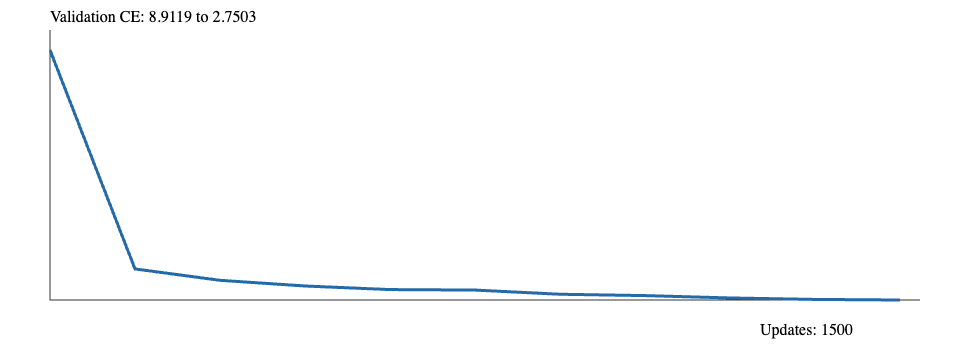
\includegraphics[width=0.88\linewidth]{../../01-basics/reports/local/loss.png}
 \caption{Fixed-window validation cross-entropy during the
 98M/1,500-update run.}
\end{figure}

Attention medians for lengths 64/128/256 are 1.0329/1.1378/1.1286 ms
for explicit attention and 0.9403/1.1120/1.1071 ms for SDPA;
observed forward/gradient errors are zero. Timing ranges overlap,
so these modest ratios should not be generalized.
With 32 prompt tokens and 64 new tokens, decoding falls from
431.405 to 390.203 ms (1.106$\times$), with identical output and
97,280 cache bytes. The two-layer width-64 benchmark model is
untrained and measures computation, not text quality.

\subsection{Scaling and post-training}

\begin{table}[t]
\centering
\caption{Fixed-budget size means over three seeds. The last row is
excluded from fitting.}
\begin{tabular}{rrl}
\toprule
Parameters & Validation CE & Use\\
\midrule
43,168 & 4.4095 & Fit\\
84,720 & 4.1777 & Fit\\
139,584 & 4.0768 & Fit\\
207,760 & 3.9630 & Fit\\
289,248 & 3.8706 & Hold-out\\
\bottomrule
\end{tabular}
\end{table}
The fitted offset is 3.328899, amplitude 1.077007, exponent 0.33,
and $N_0=43,168$. The held-out prediction is 3.903813 versus
observed 3.870621: 0.8575\% relative error.

\begin{table}[t]
\centering
\caption{Constrained numeric-task accuracy. Times cover training
loops only, averaged over seeds.}
\begin{tabular}{lrrrrr}
\toprule
Method & Seed 42 & Seed 43 & Seed 44 & Mean & Seconds\\
\midrule
SFT & 85\% & 95\% & 90\% & 90\% & 2.751\\
DPO & 95\% & 90\% & 85\% & 90\% & 3.599\\
RLVR & 85\% & 85\% & 85\% & 85\% & 3.418\\
\bottomrule
\end{tabular}
\end{table}
The base scores 5\%. Each RLVR seed samples 64,000 answers.
The split places the unique answer-zero pair $(0,0)$ in the test set;
zero is therefore absent from positive training labels. All branches
miss that pair. Other errors include SFT predicting 5 for
$\max(6,5)$ and RLVR predicting 2 for $\max(2,8)$.
The 20-question test set limits the precision of method comparisons.

\subsection{Verified agent and self-review}

\begin{table}[t]
\centering
\caption{Successful episodes out of 12 per horizon. Noise denotes a
separate 10\% draft-action corruption test.}
\begin{tabular}{lrrrr}
\toprule
Policy / setting & 1 goal & 4 goals & 8 goals & 16 goals\\
\midrule
Before agent training & 0 & 0 & 0 & 0\\
Trajectory SFT & 12 & 12 & 12 & 12\\
SFT + environment RL & 12 & 12 & 12 & 12\\
SFT + RL + self-review & 12 & 12 & 12 & 12\\
Noise, no review & 9 & 2 & 2 & 0\\
Noise, self-review & 12 & 12 & 12 & 12\\
\bottomrule
\end{tabular}
\end{table}
Successful 16-goal episodes average 68.08 tool actions. Ordinary
self-review does not improve success and doubles calls from 68.08 to
136.17 on average. Its robustness benefit is measured under the specified
draft-action corruption process.
A saved eight-goal self-review trajectory completes 32 actions and
matches every final target; its full observations, drafts, actions,
and feedback are replayable.

\section{Limitations and reproducibility}

The 98M data budget is small and its generations remain weak.
Fixed validation windows overlap and are not full-set evaluations.
The XML collection contains only 16 selected articles, and two are
discarded for malformed templates. Size pilots are far from
convergence; a good local prediction does not validate a billion-scale
extrapolation. Alignment uses single-token constrained responses on
a tiny domain. Agent evaluation reuses known digit states in new goal
sequences; it is not open-ended filesystem, web, or software-engineering
agency. It shows a learned finite-domain controller executing long
action chains. There is no measured incremental agent reward-learning
benefit beyond imitation here, and no Triton or multi-GPU result.

Every stage includes commands, JSON records, and experiment screenshots.
Data bundles include attribution,
transformations, and SHA-256 manifests. Small checkpoints are bundled
in Git; the two roughly 1.18 GB stage-one checkpoints are uploaded to
the same repository's GitHub Releases.
A replay demo reloads a neural policy and checks final environment states.
The repository is available at
\url{https://github.com/zongyangbigpolo/AdvancedMachineLearningTask}.

\paragraph{Acknowledgment.}
GitHub Copilot assisted implementation, execution, and report drafting.

\begin{thebibliography}{9}
\bibitem[jackmcgradylee(2026)]{referenceproject}
jackmcgradylee. From Token to Agent. Public learning repository,
revision \texttt{ca6f586}, 2026.
\url{https://github.com/jackmcgradylee/from-token-to-agent}.

\bibitem[Stanford CS336(2026)]{cs336}
Stanford CS336. Language Modeling from Scratch: Systems, Scaling,
and Alignment assignments, 2026.
\url{https://github.com/stanford-cs336}.

\bibitem[Eldan and Li(2023)]{tinystories}
Ronen Eldan and Yuanzhi Li.
TinyStories: How Small Can Language Models Be and Still Speak
Coherent English? 2023. \url{https://arxiv.org/abs/2305.07759}.

\bibitem[Kaplan et~al.(2020)]{kaplan}
Jared Kaplan et~al. Scaling Laws for Neural Language Models. 2020.
\url{https://arxiv.org/abs/2001.08361}.

\bibitem[Rafailov et~al.(2023)]{dpo}
Rafael Rafailov et~al. Direct Preference Optimization: Your Language
Model is Secretly a Reward Model. 2023.
\url{https://arxiv.org/abs/2305.18290}.

\bibitem[Williams(1992)]{williams}
Ronald J. Williams. Simple statistical gradient-following algorithms
for connectionist reinforcement learning. Machine Learning,
8:229--256, 1992. \url{https://doi.org/10.1007/BF00992696}.
\end{thebibliography}
\end{document}
